\begin{figure}%[htbp]
  \begin{subfigure}[b]{.49\textwidth}
   \centering
   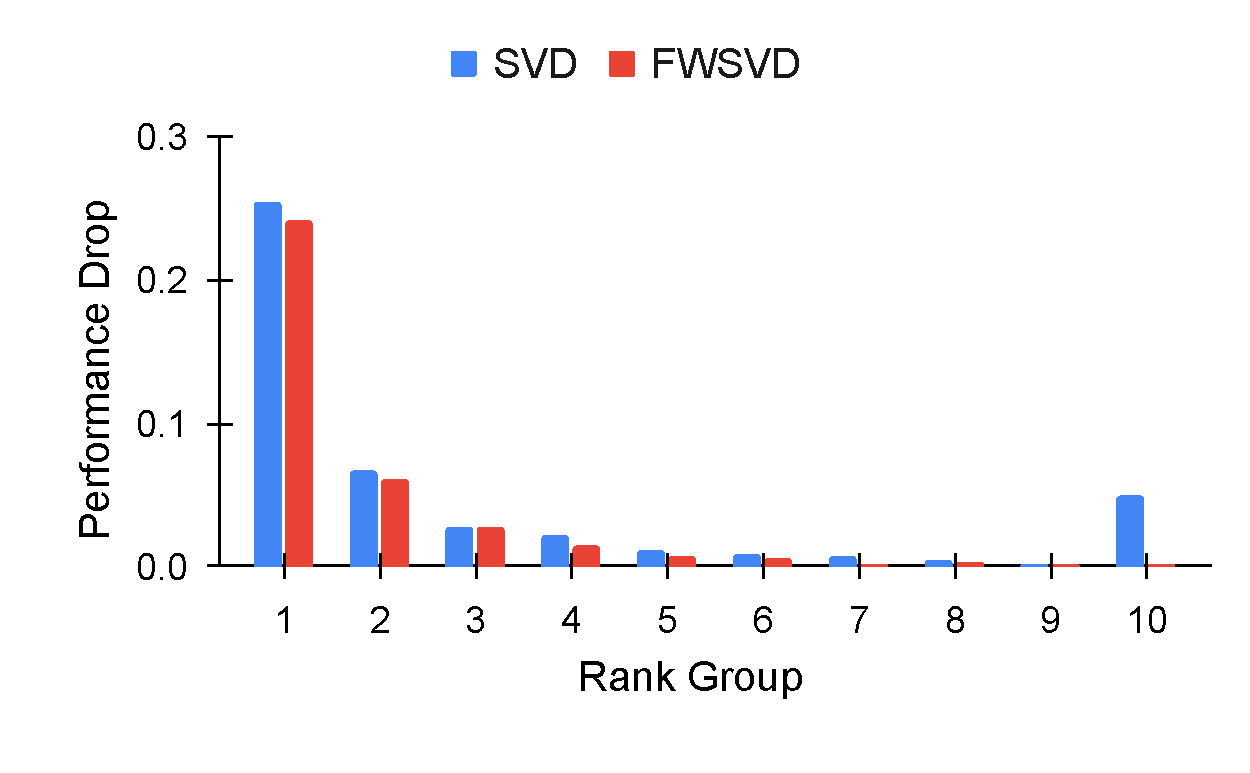
\includegraphics[clip, trim=0cm 0.5cm 0cm 0.5cm, width=\textwidth]{figures/exp_fig2_per_recolor.pdf}
       \caption{STS-B performance drop}
       \label{fig:remove_group:drop}
       \end{subfigure}
\begin{subfigure}[b]{.49\textwidth}
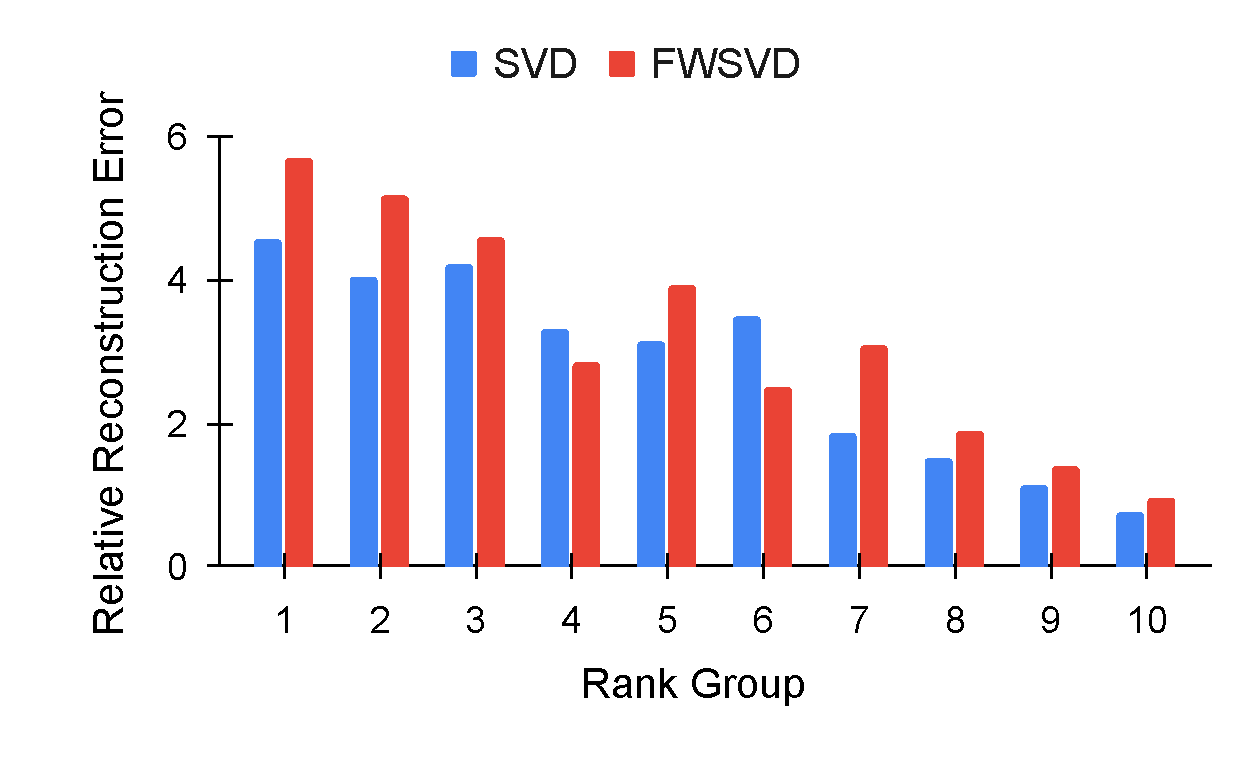
\includegraphics[clip, trim=0cm 0.5cm 0cm 0.5cm, width=\textwidth]{figures/exp_fig2_err_recolor.pdf}
\centering
  \caption{ STS-B reconstruction error}
   \label{fig:remove_group:error}
\end{subfigure}
\caption{
Results of grouped rank truncation on STS-B task. 
% More comparisons on other tasks are presented in Figure \ref{app:err_per} in Appendix.  
In (a), FWSVD shows a consistent trend of having less performance drop with the small singular value groups (group 10 has the smallest singular values), mitigating the issue of Figure \ref{fig:method_rank}. In (b), FWSVD results in a larger reconstruction error with almost all truncated groups, although FWSVD retains the model accuracy better than SVD.
% Unlike SVD, the performance drop of our FWSVD perfectly imitates the ideal trending shown in Figure \ref{fig:method_rank}. 
% \vspace{-0.5cm}
}
\label{fig:remove_group}
\end{figure}